\capitulo{3}{Conceptos teóricos}

\section{Espacios de color }
El color que percibimos en los objetos que nos rodean depende de la radiación reflejada en ellos.Según los estudios nosotros como humanos tenemos un rango ``de luz visible'' ese rango son en verdad tres frecuencias diferentes dentro del rango 769THz a 384THz.\\
Por lo que en verdad una imagen que percibimos es la unión de las tres frecuencias diferentes y para poder simular este hecho las maquinas simulan esta capacidad innata de los humanos creando los espacios de color que son modelos matemáticos para representar en una maquina lo que veríamos.\ref{fig:3.1}

\begin{figure}[h]
\centering
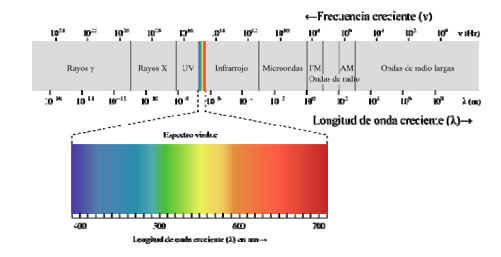
\includegraphics[width=.9\textwidth]{EspacioDeColor}
\caption{Frecuencias de luz visible \cite{Manual:HAE}}
\label{fig:3.1}
\end{figure}

\subsection{RGB}
El modelo RGB es usado por todos los sistemas digitales para la representación y captura de imágenes.\\
Se divide en tres canales:\ref{fig:3.2}\\
\begin{itemize}
	\item R: canal del rojo (RED) contiene la intensidad de rojo de cada pixel\\
	\item G: canal del verde (GREEN)contiene la intensidad de verde de cada pixel\\
	\item B: canal del azul (BLUE)contiene la intensidad de azul de cada pixel\\
\end{itemize}

\begin{figure}[h]
\centering
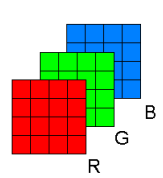
\includegraphics[width=.3\textwidth]{RGB_Canales}
\caption{Los tres canales del espacio RGB \cite{Manual:HAE}}
\label{fig:3.2}
\end{figure}
La combinación de estos colores crea todas la gama de colores representable.
El valor de la intensidad de cada canal depende de la codificación usada para su representación (8bits dan 16millones de colores)\ref{fig:3.3}

\begin{figure}[h]
\centering
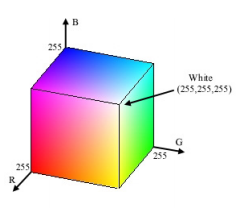
\includegraphics[width=.3\textwidth]{RGB}
\caption{Representación del modelo RGB\cite{Manual:HAE}}
\label{fig:3.3}
\end{figure}

\subsection{HSV}
El modelo HSV \cite{modelo:hsv} esta orientado a la descripción de los colores en términos mas prácticos para el ser humano que el RGB.\\
Ya que los canales significan algo por si solos no solo la cantidad de un color que no nos informa de mucho.\ref{fig:3.4}
 
\begin{itemize}
	\item H: (Matiz) que representa el tono o color.\\
	\item S: (Saturación) representa el nivel de saturación de un color.\\
	\item V: (Brillo) representa la intensidad lumínica.\\
\end{itemize}
\begin{figure}[h]
\centering
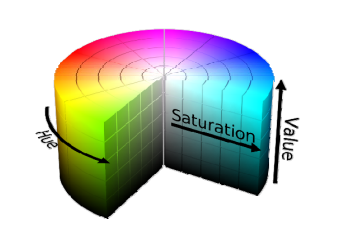
\includegraphics[width=.35\textwidth]{HSV}
\caption{Representación del modelo HSV\cite{Manual:HAE}}
\label{fig:3.4}
\end{figure}
Una ventaja con otros espacios de color parecidos es que este permite representar todas las combinaciones del espacio RGB.

\section{Transformada de hough }

\subsection{Introducción}

Uno de los puntos relevantes del proyecto es la detección de las lineas pintadas o detectadas por el algoritmo (modo automático) para ello vamos a usar una técnica que sirve para detectar formas dentro de imágenes en visión artificial siempre que puedan ser expresadas de forma matemática.

Esta tecnica fue inventada por Richard Duda y Peter Hart en 1972 pero 10 años antes Paul Hough propuso y patento \cite{pat:patHough} la idea inicial de detectar lineas en la imagen. Mas tarde se generalizo para detectar cualquier figura.

\subsection{Teoría}

Normalmente para detectar figuras sencillas en una imagen primero hay que usar algún algoritmo de detección de bordes o una binarización de la imagen, quedándonos con la región de interés apropiada (los pixeles que forman las rectas) pero normalmente faltan pixeles por el ruido en la imagen.

Para ello el metodo de hough propone solucionar el problema detectando grupos de puntos que forman los bordes de la misma figura y asi conseguir unirlos creando la recta real a la que pertenecen.

\subsection{Psudocódigo Transformada de Hough}
\ref{alg:Hough}

%Hough
\begin{algorithm*}
\DontPrintSemicolon
\KwIn{Imagen}
\KwOut{(list) de segmentos encontrados }

%$ S = \varnothing $

\ForEach {punto en la imagen}{
		\If {punto \textbf{(x,y)} esta en un borde:}{
			\ForEach {angulo en angulos $\Theta$ }{
				Calcular $\rho$  para el punto (x,y) con angulo $\Theta$ \;
				Incrementar la posicion ($\rho$ , $\Theta$ ) en el acumulador\;
			}
		}
}
Buscar las posiciones con mayores valores en el acumulador\;	

\Return {$Las rectas cuyos valores son los mayores en el acumulador$}
\label{alg:Hough}
\end{algorithm*}

\subsection{Limitaciones}
Para que este proceso sea exitoso los bordes del objeto deben ser detectados bien con un buen pre-procesado de la imagen y aparecer claramente las nubes de puntos que forman las rectas.\ref{fig:3.5}

\begin{figure}[h]
\centering
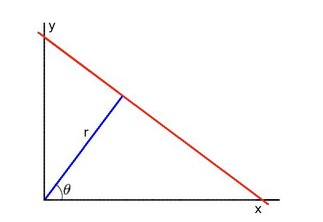
\includegraphics[width=.3\textwidth]{hough}
\caption{Lineas de hough\cite{opencv:houghIm}}
\label{fig:3.5}
\end{figure}
\subsection{Transformada probabilística de Hough}



\cite{Kiryati20001157}Es una version que se basa en que la detección de bordes o la producción de la imagen binaria que contiene el objeto, podría tener ruido y por lo tanto los pixeles que corresponden al ruido con la transformada normal podrían ser considerados como una recta, cuando en verdad es ruido.\\
Para que unos puntos sean considerados recta en la probabilística el numero necesario de ellos es menor que en la normal. Pero penalizando a los puntos que se consideran la nube de puntos aleatoria a aquellos que estén en duda de donde se colocan.\\
Un exceso de ruido en la imagen también haría este método inservible pero para pequeñas cantidades lo hacen mas preciso que el método normal.
Otra ventaja es que con este método obtenemos el segmento que necesitamos no la prolongación de el hasta el infinito.

\section{Skeletonize }
\cite{scik:skeleton} Dentro del pre-procesado de la imagen uno de los puntos clave para que nuestro método funcione es que después de su binarización y la detección de los bordes de la imagen a procesar debemos reducir la región sobre la que aplicar la transformada de hough para que esta sea mas rápida y detecte menos número de lineas imaginarias por cada linea real.

Esto lo conseguiremos usando una función de esqueletonizado que nos devuelve lo que su nombre indica el esqueleto de los bordes de la imagen reducidos a 1 pixel.\ref{fig:3.6}


\begin{figure}
\begin{subfigure}[b]{.5\linewidth}
\centering\large 
\includegraphics[width=.9\textwidth]{skeletonizeA}
\caption{Original}
\end{subfigure}%
\begin{subfigure}[b]{.5\linewidth}
\centering\large 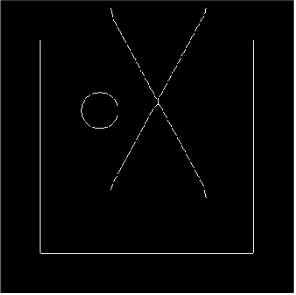
\includegraphics[width=.9\textwidth]{skeletonizeB}
\caption{Skeletonizada}
\end{subfigure}
\caption{Ejemplo de eskeletonize.}\label{fig:3.6}
\end{figure}


\section{Grafos}
	
\subsection{Introducción}
\subsection{K-componentes}